\documentclass{article}
\usepackage[utf8]{inputenc}
\usepackage{tabularx} % extra features for tabular environment
\usepackage{amsmath}  % improve math presentation
\usepackage{graphicx} % takes care of graphic including machinery
\usepackage{xspace}
\usepackage{tikz}
\usepackage{enumitem}
\usetikzlibrary{babel}
\usepackage[american]{circuitikz}
\usetikzlibrary{calc}
\usepackage{float}
\usepackage{siunitx}
\usepackage{pgfplots}
\usepackage[skins,theorems]{tcolorbox}
\tcbset{highlight math style={enhanced,
  colframe=red,colback=white,arc=0pt,boxrule=1pt}}
\pgfplotsset{width=10cm,compat=1.9}
\usepackage[margin=1in,letterpaper]{geometry} % decreases margins
\usepackage{cite} % takes care of citations
\usepackage[final]{hyperref} % adds hyper links inside the generated PDF file
\hypersetup{
colorlinks=true,       % false: boxed links; true: colored links
linkcolor=blue,        % color of internal links
citecolor=blue,        % color of links to bibliography
filecolor=magenta,     % color of file links
urlcolor=blue        
}

\begin{document}

\title{{\textbf{ASSIGNMENT 5}}}
\author{\textbf{TADIPATRI UDAY KIRAN REDDY}\\\textbf{EE19BTECH11038}}
\maketitle

\section*{\hfil Problem 1}
Effective $Q_{eff} = Q_1 + Q2$, where $Q_i = \sqrt{\frac{R_{out}}{R_{in}} - 1}$. Since this is 2 stage low pass matching network let us take a intermediate jump of resistance $R_i$.
\begin{gather}
	Q_1 = \sqrt{\frac{R_{HI}}{R_{i}} - 1} = \frac{\omega L_1}{R_{i} + R_{rs_1}} = \omega C_1 R_{HI}\\
	Q_2 = \sqrt{\frac{R_{i}}{R_{LO}} - 1} = \frac{\omega L_2}{R_{LO} + R_{rs_2}} = \omega C_2 R_{i}
\end{gather}
The loss in the network is because of lossy inductors which have a Q of 20.\\
\begin{gather}
	\eta = \frac{P_L}{P_L + P_{rs_1} + P_{rs_2}} = \frac{P_L}{P_L + \frac{E_{L_1} + E_{L_2}}{Q}}\\
	\eta = \frac{P_L}{P_L + \frac{Q_1P_I + Q_2P_L}{Q}} = \frac{1}{1 + \frac{Q_1\frac{P_I}{P_L} + Q_2}{Q}}
\end{gather}
Here $\frac{P_I}{P_2}$ is inverse of efficiency of only 2nd stage which is $1 + \frac{Q_2}{Q}$. Therefore,
\begin{gather}
	\eta = \frac{1}{1 + \frac{Q_1 + Q_2 + Q_1Q_2/Q}{Q}}\\
	max\{\eta\} \iff min\{Q_1 + Q_2 + Q_1Q_2/Q\}\\
	\implies \frac{\partial}{\partial R_i}\left(Q_1 + Q_2 + Q_1Q_2/Q\right) = 0\\
	Q(\frac{\partial Q_1}{\partial R_i} + \frac{\partial Q_2}{\partial R_i}) + Q_1\frac{\partial Q_2}{\partial R_i} + Q_2\frac{\partial Q_1}{\partial R_i} = Q\left[-\frac{R_{HI}}{2R_i^2Q_1} + \frac{1}{2R_{LO}Q_2}\right] + Q_1\left[\frac{1}{2R_{LO}Q_2}\right] - Q_2\left[\frac{R_{HI}}{2R_i^2Q_1}\right]=0\\
\end{gather}
Simplifying the above equation we end up getting,
\begin{gather}
R_i^2Q_1(Q_1 + Q) = R_{HI}R_{LO}Q_2(Q_2 + Q)
\end{gather}
Assuming $Q_2, Q_1 << Q$,
\begin{gather}
2R_i^2Q_1Q = R_{HI}R_{LO}Q_2Q\\
\implies 4R_i^4 - R_{HI}R_i^3 + R_{HI}^2R_{LO}R_i - R_{HI}^2R_{LO^2} = 0\\
\implies R_i = 223.6, 52.7, 947.213
\end{gather}
\begin{figure}[H]
	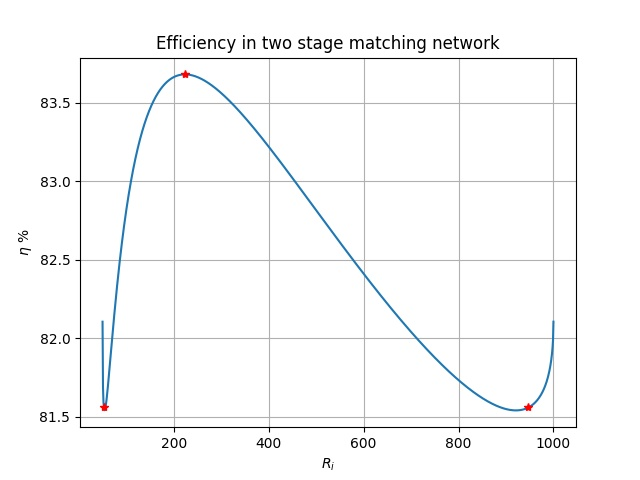
\includegraphics[scale=0.8]{./figs/plot.jpg}
\end{figure}
Plugging in these values in the equation (3) we get highest value for R=223.6
\begin{gather}
\implies \tcbhighmath[drop fuzzy shadow]{R_i = 223.6}\\
\implies \tcbhighmath[drop fuzzy shadow]{Q_1 = 1.863, Q_2 = 1.863}
\end{gather}
From equation (5) we get,
\begin{equation}
	\tcbhighmath[drop fuzzy shadow]{\eta = 83.69 \%}
\end{equation}
From equation (1) and (2) we get,
\begin{gather}
	L_1 = Q_1\frac{R_i + \omega L_1/Q}{\omega}\\
	\implies L_1 = \frac{R_i}{\omega (1/Q_1 - 1/Q)}\\
	\tcbhighmath[drop fuzzy shadow]{L_1 = 73.1nH}\\
	L_2 = \frac{R_{LO}}{\omega (1/Q_2 - 1/Q)}\\
	\tcbhighmath[drop fuzzy shadow]{L_2 = 16.35nH}\\
	C_1 = \frac{Q_1}{\omega R_{HI}}\\
	\tcbhighmath[drop fuzzy shadow]{C_1 = 0.29fF}\\
	C_2 = \frac{Q_2}{\omega R_{i}}\\
	\tcbhighmath[drop fuzzy shadow]{C_2 = 1.3fF}
\end{gather}
%Power efficiency of below matching circuit can be found as,
%% fig
%%
%\begin{gather}
%P = VI^*\\
%P_{in} = V_{in}{\frac{V_{in}^*}{Z_{in}^*}} = |V_{in}|^2\left(\frac{s^2LC + sRC + 1}{sL + R}\right)^*\\
%P_{out} = \frac{V_{in}R}{sL + R}\frac{V_{in}^*}{(sL + R)^*} = |V_{in}|^2\frac{R}{|sL + R|^2}\\
%Efficiency = \eta = \frac{|P_{out}|}{|P_{in}|}\\
%\eta = \frac{\frac{R}{|sL + R|^2}}{\frac{|s^2LC + sRC + 1|}{|sL + R|}} = \frac{R}{|sL+R||s^2LC + sRC + 1|}
%\end{gather}

\section*{\hfil Problem 2}
\subsection*{(a)}
\begin{figure}[H]
	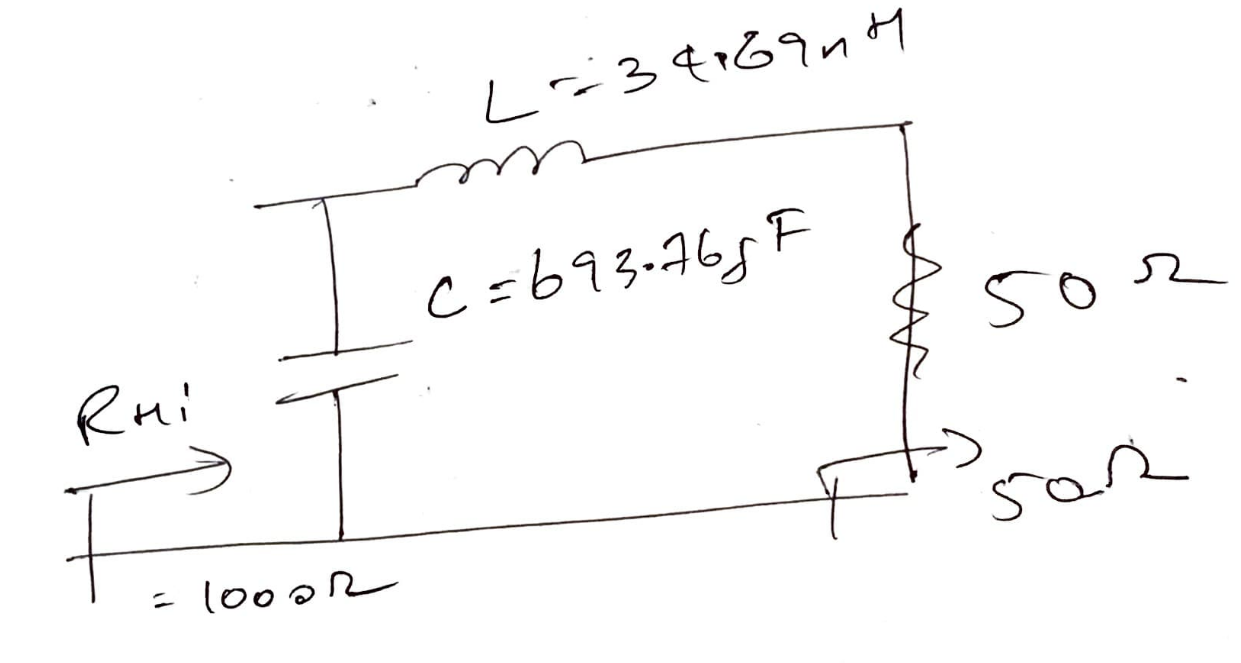
\includegraphics[scale=0.2]{./figs/q2_a.png}
\end{figure}
$R_{HI} = 1000 \si{\ohm}, R_{LO} = 50 \si{\ohm}; \omega = 2 \pi 10^9$
\begin{gather}
	Q = \sqrt{\frac{1000}{50} - 1} \implies \tcbhighmath[drop fuzzy shadow]{Q = 4.359} \\
	Q = \frac{\omega L}{R_{LO}} \implies \tcbhighmath[drop fuzzy shadow]{L = 34.69 nH} \\
	Q = \omega CR_{Hi} \implies \tcbhighmath[drop fuzzy shadow]{C = 693.76fF}
\end{gather}
\subsection*{(b)}
Given $Q_{loaded} = 5$ which means Q of network is 10. 
\subsubsection*{(i) Low-pass $\Pi$}
\begin{figure}[H]
	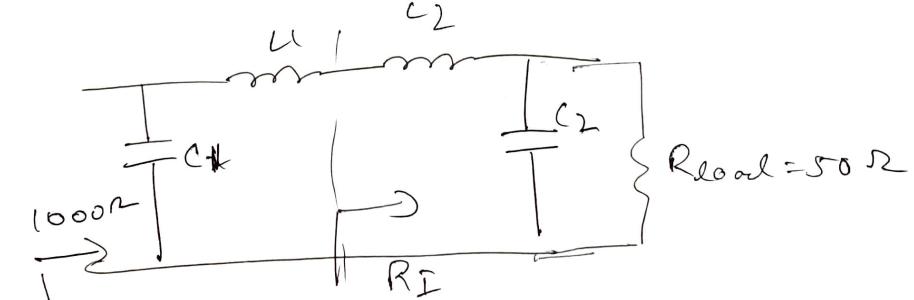
\includegraphics[scale=0.4]{./figs/q2_bii.png}
\end{figure}
\begin{gather}
	Q_1 = \sqrt{\frac{1000}{R_{I}}-1}\\
	Q_2 = \sqrt{\frac{50}{R_{I}}-1}\\
	Q = \sqrt{\frac{1000}{R_{I}}-1} + \sqrt{\frac{50}{R_{I}}-1} = 10\\
	\implies 104R_I^2 -2100R_I + 9025 = 0
	\implies \tcbhighmath[drop fuzzy shadow]{R_I = 13.99 \si{\ohm}}
\end{gather}

\subsubsection*{(i) Low-pass T}
\begin{figure}[H]
	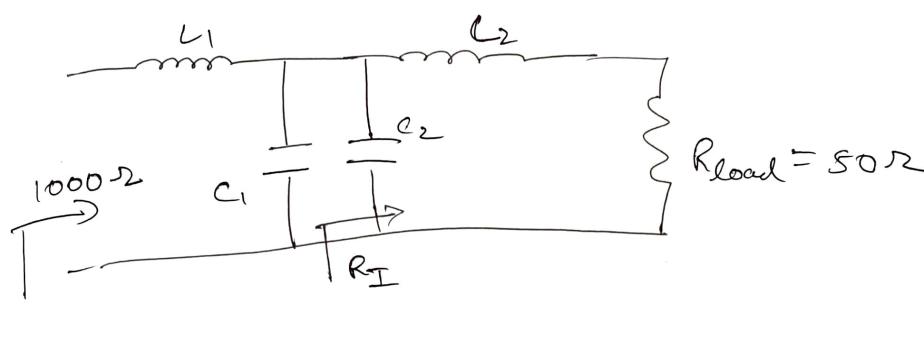
\includegraphics[scale=0.4]{./figs/q2_bi.png}
\end{figure}
\begin{gather}
	Q_1 = \sqrt{\frac{R_I}{R_{HI}}-1}\\
	Q_2 = \sqrt{\frac{R_I}{R_{LO}}-1}\\
	Q = \sqrt{\frac{R_I}{1000}-1} + \sqrt{\frac{R_I}{50}-1} = 10\\
	\implies R_I^2(3.61e-4) - 4.2R_I + 10400 = 0\\
	\tcbhighmath[drop fuzzy shadow]{R_I = 3574.26 \si{\ohm}}
\end{gather}
\end{document}